\section{Results}

We examine the true positive ($\TPR$) and false positive ($\FPR$) rates, $\TPR = \TP / \operatorname{P}$ and $\FPR = \FP / \operatorname{N}$, where $\TP$ is the number of correctly predicted users with high income, $\operatorname{P}$ is the total number of users with high income, $\FP$ is the number of users incorrectly classified as having high income, and $\operatorname{N}$ is the total number of users with low income.

\begin{figure}[ht]
\begin{center}
{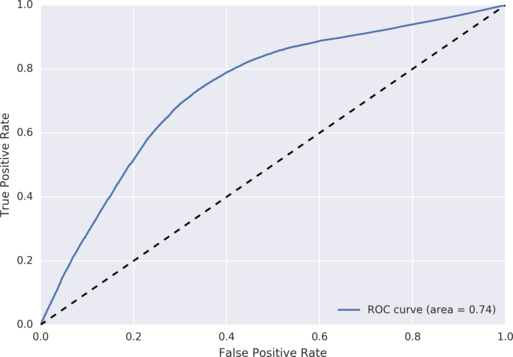
\includegraphics[width=0.9\columnwidth]{ROC_Beta_based_approach_201504.png}}
\caption{ROC curve for prediction procedure. We observed an $\AUC = 0.74$ indicating that our predictor is better than a random predictor ($\AUC \simeq 0.50$). We plot the ROC (\textit{Receiver Operating Characteristic}) curve, showing $\TPR$ and $\FPR$ for the set of possible values of $\tau$. We see that our methodology clearly outperforms random guessing (dashed straigh line). We can summarize our performance by calculating  the $\AUC$ (\textit{Area Under the Curve}) which in Figure~\ref{ROC_multiclass} is $\AUC = 0.74$. Note that random guessing would give a value of $\AUC \simeq 0.50$.
}

\label{ROC_multiclass}
\end{center}
\end{figure}

Alternatively we can evaluate the performance of our model by computing its accuracy for a given threshold $\tau$ of $\FPR$, computed as the ratio between $\TP$ and $\TN$ over the total polulation for a certain $\FPR$. The best accuracy obtained is \num{0.71} for $\tau = 0.4$, as shown in figure~\ref{fig:accuracy_vs_fpr}.

\begin{figure}[ht]
\begin{center}
{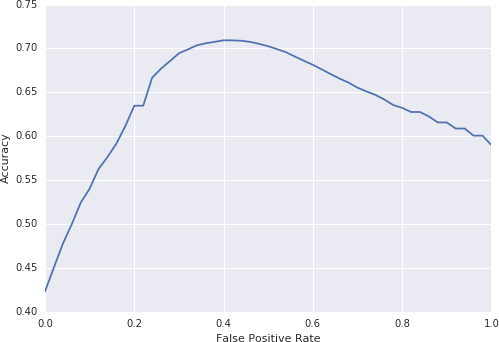
\includegraphics[width=0.9\columnwidth]{accuracy_vs_fpr.png}}
\caption{Accuracy as a function of FPR\@. The best accuracy obtained is 0.71.}
\label{fig:accuracy_vs_fpr}
\end{center}
\end{figure}

\subsection{Comparison with other inference methods}

We applied two other inference methods to the same data and compared their accuracies to our Bayesian model.

\begin{itemize}
	\item \textbf{Random selection} which chooses randomly the category for each user.
	\item \textbf{Majority voting} which decides whether a user is in the high or low income category depending on the category of the majority of its contacts. In case of a tie, the category is chosen randomly.
\end{itemize}

The accuracy of the first method is as expected \num{0.50}, while the accuracy for majority voting is \num{0.66}. This is significantly worse than the accuracy we get with the Bayesian Method.
